%!TEX root = uist14.tex
\section{Iteration 3: Head motion refinement}
\label{sec:iteration-3:-head}
\subsection{Problem Statement and Goal}
Both {\em Naive IR} and {\em Intensity IR} rely on list navigation on the
near-eye display for the refinement step. The list interface has a few clear shortcomings: navigation actions map poorly to real world results, and the users must switch their focus back and forth between the physical scene and the near-eye display. These problems motivated us to design an approach that harnesses the head orientation during the {\em refinement} stage.

In our third iteration, we build a system which further minimizes the chance of
falling back to list based {\em refinement}.

\subsection{Technique}

We introduce a third technique that uses a combination of motion sensors and IR to learn the relative orientations of
targets in a room and intelligently suggest targets during refinement (see
Figure~\ref{fig:third_technique}).

Unfortunately, this absolute orientation cannot be applied to all indoor
environments, since the user’s movements through the space could change the relationships between targets. However, with the constraint that the targets are spread around the periphery, their relative orientations are stable
(see Figure~\ref{fig:third_principle}). 

\begin{figure}[t]
\centering
\includegraphics[width=1\columnwidth]{figures/third_principle.png}
\caption{Even when the user's absolution position changes, the relative relationship in the orientation space remain invariant.}
\label{fig:third_principle}
\end{figure}

\begin{figure}[t]
\centering
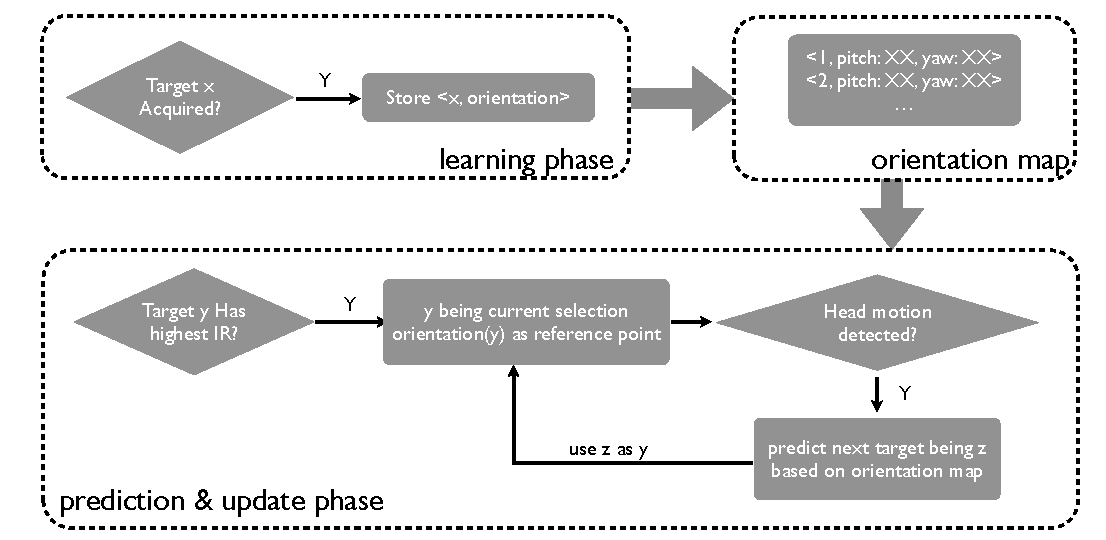
\includegraphics[width=1\columnwidth]{figures/third_technique3.pdf}
\caption{\ben{figure in interactionModel2.key file.} Our third technique learned each target's absolute orientation and construct the orientation map. Though we store the absolute orientation value, during the {\em refinement} stage, the prediction is only based on relative changes to a reference point. In such a way, the prediction will work regardless of user's position.}
\label{fig:third_technique}
\end{figure}

In the learning stage, the user scans over the targets, and the
system attains the absolute orientation of each device from IR and motion sensors. From this information it can abstract out their relative positions and build an {\em adjacency map}.

After the map is created, the user can hold down on the touchpad to enter a
quasi-mode for refinement. In this quasi-mode, one device lights up at a time. When the user turns his head in the direction of another device, the light switches to that device. Therefore, the user can move between devices one at a time with slight head movements. We implement this interaction by calculating the user's direction of motion using a low-passed history of sensor measurements and searching through the adjacency map for
the nearest device in that direction. 

\subsection{Evaluation}
\ben{We then need evaluation results here, quantitative and qualitative.}
\bjoern{got to here in my pass}


% %!TEX root = uist14.tex
% \section{Iteration 3: Orientation-based refinement}
% \bjoern{While taking IR intensity into account further reduced the need for manual refinement and increased performance, the UI navigation scheme is problematic - it is not spatially related in any meaningful way to the layout of targets in a room. A better interaction technique would respect that ordering. For example, when refinement is needed, tilting the head slightly to the right could select the target that's adjacent to the right of the currently selected target.

% Such spatial navigation requires knowledge about the layout of targets in the environment. However, one of the strengths of our technique so far is that it does not require any map ahead of time. To enable some spatial navigation, we introduce a final iteration in which we build up a spatial data structure by demonstration (i.e., the user looks around the room) and then leverage that data structure during the refinement step of our interaction.}

% \bjoern{This technique is based on the assumption that users will generally select targets in indoor environments where targets are spread around the periphery. These assumptions enable us to use orientation data without knowing the user's absolute position.}

% \subsection{Implementation}
% \bjoern{give implementation details}

% \subsection{Informal User Feedback}
% \bjoern{We informally evaluate this technique with N users: ...}

 
%%% Local Variables: 
%%% mode: latex
%%% TeX-master: "uist14"
%%% End: 
